%Version 2.1 April 2023
% See section 11 of the User Manual for version history
%
%%%%%%%%%%%%%%%%%%%%%%%%%%%%%%%%%%%%%%%%%%%%%%%%%%%%%%%%%%%%%%%%%%%%%%
%%                                                                 %%
%% Please do not use \input{...} to include other tex files.       %%
%% Submit your LaTeX manuscript as one .tex document.              %%
%%                                                                 %%
%% All additional figures and files should be attached             %%
%% separately and not embedded in the \TeX\ document itself.       %%
%%                                                                 %%
%%%%%%%%%%%%%%%%%%%%%%%%%%%%%%%%%%%%%%%%%%%%%%%%%%%%%%%%%%%%%%%%%%%%%

\documentclass[sn-nature,referee,pdflatex]{sn-jnl}

%%%% Standard Packages
%%<additional latex packages if required can be included here>

\usepackage{graphicx}%
\usepackage{multirow}%
\usepackage{amsmath,amssymb,amsfonts}%
\usepackage{amsthm}%
\usepackage{mathrsfs}%
\usepackage[title]{appendix}%
\usepackage{xcolor}%
\usepackage{textcomp}%
\usepackage{manyfoot}%
\usepackage{booktabs}%
\usepackage{algorithm}%
\usepackage{algorithmicx}%
\usepackage{algpseudocode}%
\usepackage{listings}%
%%%%

%%%%%=============================================================================%%%%
%%%%  Remarks: This template is provided to aid authors with the preparation
%%%%  of original research articles intended for submission to journals published
%%%%  by Springer Nature. The guidance has been prepared in partnership with
%%%%  production teams to conform to Springer Nature technical requirements.
%%%%  Editorial and presentation requirements differ among journal portfolios and
%%%%  research disciplines. You may find sections in this template are irrelevant
%%%%  to your work and are empowered to omit any such section if allowed by the
%%%%  journal you intend to submit to. The submission guidelines and policies
%%%%  of the journal take precedence. A detailed User Manual is available in the
%%%%  template package for technical guidance.
%%%%%=============================================================================%%%%

\usepackage{comment}
\usepackage{anyfontsize}
\usepackage[style=default]{caption}
\usepackage{float}
\usepackage{placeins}
\usepackage{booktabs}
\usepackage{longtable}
\usepackage{array}
\usepackage{multirow}
\usepackage{wrapfig}
\usepackage{float}
\usepackage{colortbl}
\usepackage{pdflscape}
\usepackage{tabu}
\usepackage{threeparttable}
\usepackage{threeparttablex}
\usepackage[normalem]{ulem}
\usepackage{makecell}
\usepackage{xcolor}


\raggedbottom



% Pandoc syntax highlighting
\usepackage{color}
\usepackage{fancyvrb}
\newcommand{\VerbBar}{|}
\newcommand{\VERB}{\Verb[commandchars=\\\{\}]}
\DefineVerbatimEnvironment{Highlighting}{Verbatim}{commandchars=\\\{\}}
% Add ',fontsize=\small' for more characters per line
\usepackage{framed}
\definecolor{shadecolor}{RGB}{248,248,248}
\newenvironment{Shaded}{\begin{snugshade}}{\end{snugshade}}
\newcommand{\AlertTok}[1]{\textcolor[rgb]{0.94,0.16,0.16}{#1}}
\newcommand{\AnnotationTok}[1]{\textcolor[rgb]{0.56,0.35,0.01}{\textbf{\textit{#1}}}}
\newcommand{\AttributeTok}[1]{\textcolor[rgb]{0.13,0.29,0.53}{#1}}
\newcommand{\BaseNTok}[1]{\textcolor[rgb]{0.00,0.00,0.81}{#1}}
\newcommand{\BuiltInTok}[1]{#1}
\newcommand{\CharTok}[1]{\textcolor[rgb]{0.31,0.60,0.02}{#1}}
\newcommand{\CommentTok}[1]{\textcolor[rgb]{0.56,0.35,0.01}{\textit{#1}}}
\newcommand{\CommentVarTok}[1]{\textcolor[rgb]{0.56,0.35,0.01}{\textbf{\textit{#1}}}}
\newcommand{\ConstantTok}[1]{\textcolor[rgb]{0.56,0.35,0.01}{#1}}
\newcommand{\ControlFlowTok}[1]{\textcolor[rgb]{0.13,0.29,0.53}{\textbf{#1}}}
\newcommand{\DataTypeTok}[1]{\textcolor[rgb]{0.13,0.29,0.53}{#1}}
\newcommand{\DecValTok}[1]{\textcolor[rgb]{0.00,0.00,0.81}{#1}}
\newcommand{\DocumentationTok}[1]{\textcolor[rgb]{0.56,0.35,0.01}{\textbf{\textit{#1}}}}
\newcommand{\ErrorTok}[1]{\textcolor[rgb]{0.64,0.00,0.00}{\textbf{#1}}}
\newcommand{\ExtensionTok}[1]{#1}
\newcommand{\FloatTok}[1]{\textcolor[rgb]{0.00,0.00,0.81}{#1}}
\newcommand{\FunctionTok}[1]{\textcolor[rgb]{0.13,0.29,0.53}{\textbf{#1}}}
\newcommand{\ImportTok}[1]{#1}
\newcommand{\InformationTok}[1]{\textcolor[rgb]{0.56,0.35,0.01}{\textbf{\textit{#1}}}}
\newcommand{\KeywordTok}[1]{\textcolor[rgb]{0.13,0.29,0.53}{\textbf{#1}}}
\newcommand{\NormalTok}[1]{#1}
\newcommand{\OperatorTok}[1]{\textcolor[rgb]{0.81,0.36,0.00}{\textbf{#1}}}
\newcommand{\OtherTok}[1]{\textcolor[rgb]{0.56,0.35,0.01}{#1}}
\newcommand{\PreprocessorTok}[1]{\textcolor[rgb]{0.56,0.35,0.01}{\textit{#1}}}
\newcommand{\RegionMarkerTok}[1]{#1}
\newcommand{\SpecialCharTok}[1]{\textcolor[rgb]{0.81,0.36,0.00}{\textbf{#1}}}
\newcommand{\SpecialStringTok}[1]{\textcolor[rgb]{0.31,0.60,0.02}{#1}}
\newcommand{\StringTok}[1]{\textcolor[rgb]{0.31,0.60,0.02}{#1}}
\newcommand{\VariableTok}[1]{\textcolor[rgb]{0.00,0.00,0.00}{#1}}
\newcommand{\VerbatimStringTok}[1]{\textcolor[rgb]{0.31,0.60,0.02}{#1}}
\newcommand{\WarningTok}[1]{\textcolor[rgb]{0.56,0.35,0.01}{\textbf{\textit{#1}}}}

% tightlist command for lists without linebreak
\providecommand{\tightlist}{%
  \setlength{\itemsep}{0pt}\setlength{\parskip}{0pt}}





\begin{document}


\title[MAP-reduction-meta]{Meaningfully reducing consumption of meat and
animal products is an unsolved problem: \newline A meta-analysis}

%%=============================================================%%
%% Prefix	-> \pfx{Dr}
%% GivenName	-> \fnm{Joergen W.}
%% Particle	-> \spfx{van der} -> surname prefix
%% FamilyName	-> \sur{Ploeg}
%% Suffix	-> \sfx{IV}
%% NatureName	-> \tanm{Poet Laureate} -> Title after name
%% Degrees	-> \dgr{MSc, PhD}
%% \author*[1,2]{\pfx{Dr} \fnm{Joergen W.} \spfx{van der} \sur{Ploeg} \sfx{IV} \tanm{Poet Laureate}
%%                 \dgr{MSc, PhD}}\email{iauthor@gmail.com}
%%=============================================================%%

\author*[1]{\fnm{Seth
Ariel} \sur{Green} }\email{\href{mailto:setgree@stanford.edu}{\nolinkurl{setgree@stanford.edu}}}

\author[1]{\fnm{Maya B.} \sur{Mathur} }

\author[2]{\fnm{Benny} \sur{Smith} }



  \affil[1]{\orgdiv{Quantitative Sciences Unit, Department of
Medicine}, \orgname{Stanford University}}
  \affil[2]{\orgname{Allied Scholars for Animal Protection}}

\abstract{Which interventions produce the largest and most enduring
reductions in consumptions of meat and animal products (MAP)? We address
this question with a theoretical review and meta-analysis of randomized
controlled trials that measured MAP consumption at least one day after
intervention. We meta-analyze 35 papers comprising 41 studies, 112
interventions, and approximately 87,000 subjects. We find that these
papers employ four major strategies to changing behavior: choice
architecture, persuasion, psychology, and a combination of persuasion
and psychology. The pooled effect of all 114 interventions on MAP
consumption is quite small (standardized mean difference {[}SMD{]} =
0.07; 95\% CI: {[}0.02, 0.12{]}), indicating an unsolved problem.
Interventions aiming to reduce only consumption of red and processed
meat were more effective: SMD = 0.25 (95\% CI: {[}0.11, 0.38{]}), but it
remains unclear whether such interventions increase consumption of other
forms of MAP. We further explore effect size heterogeneity by approach,
population, and study features. We conclude that while no theoretical
approach provides a proven remedy to MAP consumption, designs and
measurement strategies have generally been improving over time, and many
promising interventions await rigorous evaluation.}

\keywords{meta-analysis, meat, plant-based, randomized controlled trial}



\maketitle

\section{Introduction}\label{sec1}

Global MAP consumption is increasing annually \citep{godfray2018} and
expected to continue doing so \citep{whitton2021}. Abating this trend is
vital to reducing chronic disease and the risk of zoonotic pandemics
\citep{willett2019, landry2023, hafez2020}, mitigating environmental
degradation and climate change
\citep{poore2018, koneswaran2008, greger2010}, and improving animal
welfare \citep{kuruc2023, scherer2019}. However, eating MAP is widely
regarded as normal, ethical, and necessary
\citep{piazza2022, milford2019}.

There is a vast and diverse literature investigating potential means to
reduce MAP consumption. Example approaches include providing free access
to meat substitutes \citep{katare2023}, changing the price
\citep{horgen2002} or perceptions \citep{kunst2016} of meat, or
attempting to persuade people to change their diets
\citep{bianchi2018conscious}. Some interventions are associated with
large impacts \citep{lentz2020, boronowsky2022, reinders2017}, and prior
reviews have concluded that some frequently studied approaches, such as
using persuasive messaging that appeals to animal welfare
\citep{mathur2021meta}, may be consistently effective. A particularly
high-profile strand of this literature employs choice architecture,
i.e.~altering the contexts in which MAP is selected
\citep{bianchi2018restructuring}, for instance by changing menu layouts
\citep{bacon2018, gravert2021}, placing vegetarian items more
prominently in dining halls \citep{ginn2024}, or making plant-based
options the default at catered meals \citep{hansen2021}. Choice
architecture has been cited as a cheap, effective way of altering
dietary behavior \citep{colgan2024}, and governments, universities, and
other institutions are increasingly implementing these approaches in
such settings as dining halls \citep{pollicino2024} and hospital
cafeterias \citep{morgenstern2024}.

However, recurring design and measurement limitations comprise this
literature. Many interventions are either not randomized
\citep{garnett2020} or underpowered \citep{delichatsios2001}. Measured
outcomes are often imperfect proxies of MAP consumption, such as
attitudes, intentions, and hypothetical choices
\citep{raghoebar2020, vermeer2010}, yet behaviors often do not track
with these psychological processes
\citep{mathur2021effectiveness, porat2024} and reported preferences
\citep{hensher2010}. Further, many studies measure only immediate rather
than long-term effects \citep{hansen2021, griesoph2021}.

In the past few years, a new wave of MAP reduction research has made
commendable methodological advances in design, measurement validity, and
statistical power. Historically, in some scientific fields, strong
effects detected in early studies with methodological limitations were
ultimately overturned by more rigorous follow-ups
\citep{wykes2008, paluck2019, scheel2021}. Does this phenomenon hold in
the MAP reduction literature as well?

To address this question, we conducted a meta-analysis of RCTs that aim
to reduce MAP consumption and that meet basic methodological standards
\citep{andersson2021, kanchanachitra2020, abrahamse2007, acharya2004, banerjee2019, bianchi2022, bochmann2017, bschaden2020, carfora2023, cooney2014, cooney2016, feltz2022, haile2021, hatami2018, hennessy2016, jalil2023, mathur2021effectiveness, merrill2009, norris2014, peacock2017, polanco2022, sparkman2021, weingarten2022, piester2020, aberman2018, aldoh2023, allen2002, camp2019, coker2022, sparkman2020, berndsen2005, bertolaso2015, fehrenbach2015, mattson2020, shreedhar2021}.
Specifically, we restricted eligibility to RCTs that measured
consumption outcomes at least a single day after treatment was first
administered and that had at least 25 subjects in both treatment and
control (or, for cluster-assigned studies, at least ten clusters in
total).

Numerous studies specifically aim to reduce consumption of red and
processed meat (RPM), rather than all MAP. Such interventions may induce
people to switch from consuming RPM to consuming other forms of MAP,
such as chicken or fish \citep{grummon2023}. While RPM is particularly
detrimental for human health and greenhouse gas emissions
\citep{abete2014, lescinsky2022}, producing other forms of MAP also has
severe externalities, such as risking zoonotic outbreaks from factory
farms \citep{hafez2020} and causing land and water pollution
\citep{grvzinic2023}. Additionally, raising chicken and fish may lead to
substantially worse outcomes for animal welfare
\citep{mathur2022ethical}. For these reasons, we specifically assessed
the relative effectiveness of interventions that aimed to reduce all MAP
consumption, versus those that aimed only to reduce RPM consumption (17
studies)
\citep{anderson2017, carfora2017correlational, carfora2017randomised, carfora2019, carfora2019informational, delichatsios2001talking, dijkstra2022, emmons2005cancer, emmons2005project, jaacks2014, james2015, lee2018, lindstrom2015, perino2022, schatzkin2000, sorensen2005, wolstenholme2020}.

Studies in our meta-analysis pursued one of four theoretical approaches:
choice architecture, psychological appeals (typically manipulations of
perceived norms around eating meat), explicit persuasion (centered
around animal welfare, the environment, and/or health), or a combination
of psychological and persuasion messages. Interventions varied in
delivery method, for example, documentary films
\citep{mathur2021effectiveness}, leaflets \citep{peacock2017},
university lectures \citep{jalil2023}, op-eds \citep{haile2021}, and
changes to menus in cafeterias \citep{andersson2021} and restaurants
\citep{coker2022, sparkman2021}. We estimated overall effect sizes as
well as effect sizes associated with different theoretical approaches
and delivery mechanisms. Although we find some heterogeneity across
theories and mechanisms, we find consistently smaller effects on MAP
consumption than previous reviews have suggested
\citep{bianchi2018restructuring, byerly2018, chang2023, harguess2020, kwasny2022, mathur2021meta, meier2022},
with some intriguing exceptions. Thus, contradicting previous reviews
that placed fewer (if any) restrictions on studies' methodological rigor
(Supplement), we conclude that meaningfully reducing MAP consumption is
an unsolved problem. However, many promising approaches still await
rigorous evaluation.

\section{Results}\label{sec2}

Our meta-analysis included 35 papers comprising 41 studies and 112
separate point estimates. Each point estimate corresponded to a distinct
intervention. The total sample size 87,000 subjects (caveat that this is
a broad approximation: many interventions were administered at the level
of day or cafeteria and did not record an N for subjects).

Because methodological quality is rapidly improving in the literature on
MAP reduction, the majority of eligible papers (18 of 35) were published
from 2020 onwards, although the earliest was published in 2002
\citep{allen2002}. Among studies where treatment was assigned to
individuals rather than to clusters (e.g., every student in a class),
the median analyzed sample size per study was 132
subjects(25\$\^{}\{\textbackslash text\{th\}\}\$--75\(^{\text{th}}\)
percentiles: 109, 208).

We found that studies' theoretical approaches could be grouped into four
categories. \textbf{Choice architecture} studies
\citep{andersson2021, kanchanachitra2020} (n = 2 studies with 3
estimates) manipulate aspects of physical environments to reduce MAP
consumption, such as by placing the vegetarian option at eye level on a
cafeteria's billboard menu \citep{andersson2021}. \textbf{Persuasion}
studies
\citep{kanchanachitra2020, aberman2018, abrahamse2007, acharya2004, banerjee2019, bianchi2022, bochmann2017, bschaden2020, carfora2023, hennessy2016, piester2020, cooney2014, cooney2016, feltz2022, haile2021, hatami2018, jalil2023, mathur2021effectiveness, merrill2009, norris2014, peacock2017, polanco2022, sparkman2021, weingarten2022}
(n = 25 studies with 77 estimates) focus on health, environmental
(usually climate change), and animal welfare reasons to reduce MAP
consumption. Such messages are often delivered through printed
materials, such as leaflets \citep{haile2021, polanco2022}, booklets
\citep{bianchi2022} articles and op-eds \citep{sparkman2021, feltz2022},
and videos \citep{sparkman2021, cooney2016, mathur2021effectiveness}.
Less common delivery methods included in-person dietary consultations
\citep{merrill2009}, emails \citep{banerjee2019}, and text messages
\citep{carfora2023}. \textbf{Psychology} studies
\citep{aldoh2023, allen2002, camp2019, coker2022, piester2020, sparkman2020}
(n = 9 studies with 12 estimates) manipulate the interpersonal,
cognitive, or affective factors associated with eating MAP. The most
common psychological intervention is centered on social norms seeking to
alter the perceived popularity of non-MAP dishes \citep{sparkman2020}.
In one study, a restaurant put up signs stating that ``{[}m{]}ore and
more {[}retail store name{]} customers are choosing our veggie options''
\citep{coker2022}. In another, a university cafeteria put up signs
stating that ``{[}i{]}n a taste test we did at the {[}name of cafe{]},
95\% of people said that the veggie burger tasted good or very good!''
\citep{piester2020}. One study told participants that people who ate
meat are more likely to endorse social hierarchy and embrace human
dominance over nature \citep{allen2002}. Other psychological
interventions include response inhibition training, where subjects are
trained to avoid responding impulsively to stimuli such as unhealthy
food \citep{camp2019}, and implementation intentions, where participants
list potential challenges and solutions to changing their own behavior
\citep{aberman2018, shreedhar2021}. Finally, some studies combines
\textbf{persuasion} approaches with \textbf{psychological} appeals to
reduce MAP consumption
\citep{aberman2018, berndsen2005, bertolaso2015, carfora2023, fehrenbach2015, hennessy2016, mathur2021effectiveness, mattson2020, piester2020, shreedhar2021}
(n = 11 studies with 20 estimates). These studies typically combine a
persuasive message with a norms-based appeal
\citep{piester2020, mattson2020} or an opportunity to pledge to reduce
one's MAP consumption \citep{mathur2021effectiveness, shreedhar2021}.

\begin{table}[!ht]
\centering
\caption{\label{tab:table_one}Meta-analytic Results Overall and by Theoretical Approach}
\centering
\begin{tabular}[t]{llllll}
\toprule
Approach & N (Studies) & N (Estimates) & SMD & 95\% CIs & $p$ val\\
\midrule
Overall & 41 & 112 & 0.07 & {}[0.02, 0.12] & .007\\
\addlinespace[0.5em]
\multicolumn{6}{l}{\textbf{Theory}}\\
\hspace{1em}Choice Architecture & 2 & 3 & 0.21 & {}[-0.99, 1.42] & .267\\
\hspace{1em}Psychology & 19 & 32 & 0.10 & {}[0, 0.2] & .054\\
\hspace{1em}Persuasion & 25 & 77 & 0.07 & {}[0.01, 0.13] & .023\\
\hspace{1em}Persuasion \& Psychology & 11 & 20 & 0.11 & {}[-0.06, 0.28] & .189\\
\addlinespace[0.5em]
\multicolumn{6}{l}{\textbf{Type of Persuasion}}\\
\hspace{1em}Animal Welfare & 16 & 65 & 0.03 & {}[-0.02, 0.07] & .189\\
\hspace{1em}Environment & 15 & 28 & 0.09 & {}[-0.03, 0.2] & .115\\
\hspace{1em}Health & 18 & 30 & 0.08 & {}[-0.01, 0.17] & .068\\
\bottomrule
\multicolumn{6}{l}{\textsuperscript{a} Studies could occupy multiple categories for both theory and type of persuasion. Note that the}\\
\multicolumn{6}{l}{Ns for Types of Persuasion draws from both Persuasion and Persuasion and Psychology studies.}\\
\end{tabular}
\end{table}

In our dataset, the pooled effect of all interventions is standardized
mean difference (SMD) = 0.07 (95\% CI: {[}0.02, 0.12{]}), p = .007, with
some heterogeneity (standard deviation of population effects \(\tau\) =
0.082). Given the pooled effect size and the estimated heterogeneity, we
estimate that 25.9\% of true effects are above SMD = 0.1, and just 8\%
are above SMD = 0.2. Stratifying by theoretical approach, pooled
estimates were similar across psychology, persuasion, and persuasion and
psychology (SMDs from 0.07 to 0.11; Table 1). Estimates may have been
somewhat larger among the choice architecture studies (SMD = 0.21) but
the sample size was much smaller (3 estimates). Within studies with a
persuasion component, pooled estimates are similar for environmental
appeals (SMD = 0.09, 15 studies with 28 estimates), and health appeals
(SMD = 0.08, 18 studies with 30 estimates), but are smaller for appeals
to animal welfare (SMD = 0.03, 16 studies with 65 estimates). We did not
conduct meta-regression for theoretical approach or type of persuasion
because studies with multiple interventions could occupy multiple
categories, and many persuasion interventions combined multiple types of
message, e.g. \citep{jalil2023} presented students with both
environmental and health reasons to reduce MAP consumption.

\begin{figure}[H]

{\centering \includegraphics{./figures/forest_plot-1} 

}

\caption{Forest plot of all meta-analyzed studies. For papers contributing multiple point estimates, the plotted point corresponds to a fixed effects meta-analysis for each paper for visual clarity. Papers employing multiple theoretical approaches are represented once per theory. Point size is inversely proportional to variance. Points are sorted within theory by estimate size. The vertical black line demarcates an effect size of zero, and the dotted line is the observed overall effect.}\label{fig:forest_plot}
\end{figure}

Table 2 displays subset analyses and average differences in effect size
by study population, region, era of publication, and delivery method.

\begin{table}[!ht]
\centering
\caption{\label{tab:table_two}Moderator Analysis Results}
\centering
\begin{tabular}[t]{lllllll}
\toprule
Study Characteristic & N (Studies) & N (Estimates) & SMD & 95\% CIs & Subset $p$ value & Moderator $p$ value\\
\midrule
\addlinespace[0.3em]
\multicolumn{7}{l}{\textbf{Outcome}}\\
\hspace{1em}Meat and animal products & 41 & 112 & 0.07 & {}[0.02, 0.12] & .007 & \textbf{ref}\\
\hspace{1em}Red and processed meat & 17 & 25 & 0.25 & {}[0.11, 0.38] & .002 & .046\\
\addlinespace[0.3em]
\multicolumn{7}{l}{\textbf{Population}}\\
\hspace{1em}University students and staff & 18 & 38 & 0.07 & {}[-0.03, 0.16] & .139 & \textbf{ref}\\
\hspace{1em}All ages & 3 & 6 & 0.04 & {}[-0.16, 0.25] & .361 & .733\\
\hspace{1em}Adults & 17 & 61 & 0.09 & {}[0.01, 0.18] & .034 & .714\\
\hspace{1em}Adolescents & 3 & 6 & 0.02 & {}[-0.4, 0.44] & .806 & .686\\
\addlinespace[0.3em]
\multicolumn{7}{l}{\textbf{Region}}\\
\hspace{1em}North America & 23 & 74 & 0.04 & {}[-0.01, 0.08] & .142 & \textbf{ref}\\
\hspace{1em}Europe & 14 & 28 & 0.14 & {}[0.02, 0.27] & .029 & .156\\
\hspace{1em}Multi-region & 1 & 4 & 0.21 & {}[0.21, 0.21] & 0 & .000\\
\hspace{1em}Asia + Australia & 2 & 5 & 0.13 & {}[-0.17, 0.43] & .116 & .220\\
\addlinespace[0.3em]
\multicolumn{7}{l}{\textbf{Publication Decade}}\\
\hspace{1em}2000s & 6 & 8 & 0.16 & {}[-0.12, 0.43] & .199 & \textbf{ref}\\
\hspace{1em}2010s & 12 & 31 & 0.07 & {}[-0.03, 0.17] & .13 & .464\\
\hspace{1em}2020s & 23 & 73 & 0.05 & {}[-0.01, 0.11] & .074 & .369\\
\addlinespace[0.3em]
\multicolumn{7}{l}{\textbf{Method of Delivery}}\\
\hspace{1em}Educational materials & 15 & 59 & 0.01 & {}[-0.04, 0.07] & .566 & \textbf{ref}\\
\hspace{1em}Online & 8 & 22 & 0.16 & {}[-0.02, 0.34] & .067 & .170\\
\hspace{1em}Dietary consultation & 2 & 2 & 0.40 & {}[-3.36, 4.15] & .409 & .441\\
\hspace{1em}In-cafeteria & 8 & 13 & 0.10 & {}[-0.04, 0.25] & .101 & .123\\
\hspace{1em}Video & 10 & 16 & 0.01 & {}[-0.05, 0.07] & .485 & .533\\
\bottomrule
\multicolumn{7}{l}{\textsuperscript{} Moderation analyses by differences in outcomes, population, region, decade of publication, and delivery method. The first p}\\
\multicolumn{7}{l}{value column tests the hypothesis that the subset of studies with a given characteristic is significantly different than an SMD}\\
\multicolumn{7}{l}{of zero. The second compares effects within a given group, with the top category set to reference.}\\
\end{tabular}
\end{table}

The 17 studies that only attempted to reduce consumption of RPM,
comprising 25 point estimates, yielded a pooled effect of SMD = 0.25
(95\% CI: {[}0.11, 0.38{]}), p = .002, \(\tau\) = 0.201. Among these
studies, we estimate that 48\% of true RPM effects are above SMD = 0.2.
We observe consistently small effects across categories of population
(all SMDs \textless{} 0.1), but more heterogeneity by region: North
America, where a majority of studies took place, had an average effect
of SMD = 0.04 vs.~a range of 0.14 to 0.21 for other locations.

\begin{comment} 
I don't like this sentence, but I am not sure what else so I am just moving on 
\end{comment}

Effect sizes have broadly been declining over time, from an average of
SMD = 0.16 in the 2000s to SMD = 0.05 in the 2020s, during which a
majority (18 of 41) of studies were published. Finally, we note a wide
array of heterogeneity of effects associated with different delivery
mechanisms, from 0.01 for both educational materials and videos, to 0.4
for dietary consultations, though this larger effect comes from just 2
studies. For each estimate, we provide two p values. The first (subset
\(p\) value) compares the effects associated with a given subset,
e.g.~all studies with an adolescent population, to a null hypothesis of
no effect. The second (moderator \(p\) value) compares the effects
within different moderator categories, with the top category in each
grouping set to be the reference level, e.g.~testing if the pooled
effect of studies taking place in Europe is significantly different than
that of studies taking place in North America.

Table 3 compares average differences by three potential sources of bias:
publication status, data collection strategy, and use of open science
practices.

\begin{table}[!ht]
\centering
\caption{\label{tab:table_three}Sensitivity Analysis Results}
\centering
\begin{tabular}[t]{lllllll}
\toprule
Study Characteristic & N (Studies) & N (Estimates) & SMD & 95\% CIs & Subset $p$ value & Moderator $p$ value\\
\midrule
\addlinespace[0.3em]
\multicolumn{7}{l}{\textbf{Publication Status}}\\
\hspace{1em}Journal article & 29 & 52 & 0.09 & {}[0.03, 0.15] & .008 & \textbf{ref}\\
\hspace{1em}Preprint or thesis & 7 & 17 & 0.08 & {}[-0.1, 0.25] & .325 & .947\\
\hspace{1em}Nonprofit white paper & 5 & 43 & -0.04 & {}[-0.11, 0.04] & .166 & .025\\
\addlinespace[0.3em]
\multicolumn{7}{l}{\textbf{Data Collection Strategy}}\\
\hspace{1em}Self-reported & 30 & 94 & 0.06 & {}[0, 0.12] & .039 & \textbf{ref}\\
\hspace{1em}Objectively measured & 11 & 18 & 0.09 & {}[-0.04, 0.22] & .111 & .335\\
\addlinespace[0.3em]
\multicolumn{7}{l}{\textbf{Open Science}}\\
\hspace{1em}None & 24 & 54 & 0.11 & {}[0.02, 0.19] & .014 & \textbf{ref}\\
\hspace{1em}Pre-analysis plan only & 5 & 5 & 0.10 & {}[-0.51, 0.7] & .498 & .625\\
\hspace{1em}Open data only & 7 & 11 & 0.01 & {}[-0.25, 0.27] & .903 & .274\\
\hspace{1em}Pre-analysis plan \& open data & 6 & 42 & 0.02 & {}[-0.08, 0.13] & .561 & .240\\
\bottomrule
\multicolumn{7}{l}{\textsuperscript{} Sensitivity analyses by publication status, data collection strategy, and open science practices. The first p value column tests}\\
\multicolumn{7}{l}{the hypothesis that the subset of studies with a given characteristic is significantly different than an SMD of zero. The second}\\
\multicolumn{7}{l}{compares effects within a given group, with the top category set to reference.}\\
\end{tabular}
\end{table}

Within different types of publication, we find broadly similar results
for journal articles and preprints/theses (SMD = 0.09 and SMD = 0.08,
respectively), and a small backlash associated with results published as
nonprofits' white papers (SMD = -0.04. Surprisingly, we do not detect
meaningful differences between studies that recorded self-reported
vs.~objectively measured outcomes (SMD = \texttt{r}self\_report\_delta`
vs SMD = 0.09, respectively). Looking at adherence to open science
practices, the largest difference is between studies that have neither
open data nor a pre-analysis plan (SMD = 0.11) and those that have just
open data (SMD = 0.01).

Figure 2 is a modified type of funnel plot \citep{mathur2020}.

\begin{figure}[H]

{\centering \includegraphics{./figures/funnel_plot-1} 

}

\caption{Significance funnel plot that relates studies' point estimates to their standard errors and compares the pooled estimate within all studies (black diamond) to the worst-case estimate (gray diamond).}\label{fig:funnel_plot}
\end{figure}

The meta-analytic mean corrected for publication bias that favors
significant, positive results was 0.01 (95\% CI: {[}-0.014, 0.033{]}), p
= 0.421 \citep{hedges1992}. A conservative estimate that accounts for
the possibility of worst-case publication bias yields an estimate of SMD
= 0.02 (95\% CI: {[}-0.01, 0.05{]}), p = .177
\citep{mathur2020, mathur2024}.

Figure 2 is a significance funnel plot \citep{mathur2020} that relates
studies' point estimates to their standard errors and compares the
pooled estimate within all studies (black diamond) to the worst-case
estimate (gray diamond).

\section{Methods}\label{sec3}

\subsection{Study selection}\label{sec3.1}

Our meta-analytic sample comprises randomized controlled trial
evaluations of interventions intended to reduce MAP consumption that had
at least 25 subjects in treatment and control (or at least 10 clusters
for studies that were cluster-assigned) and that measured MAP
consumption at least a single day after treatment begins. We required
that studies have a pure control group receiving no treatment. We
further restricted our search to studies that were publicly circulated
in English by December 2023. We also made three decisions regarding
study inclusion after data collection began. First, we counted and
analyzed reductions in RPM separately. Second, we excluded studies that
did not aim to reduce either all MAP or all RPM consumption and instead
only sought to induce substitution from one kind of MAP to another,
e.g.swapping red meat for fish. Third, we excluded studies with
involuntary reductions, i.e.~interventions in institutions where
subjects were simply served more vegetables on their plate.

Given our interdisciplinary research question and previous work
indicating a large grey literature \citep{mathur2021meta}, we designed
and carried out a customized search process. We: 1) reviewed 157 prior
reviews, nine of which yielded included articles
\citep{mathur2021meta, bianchi2018conscious, bianchi2018restructuring, ammann2023, chang2023, DiGennaro2024, harguess2020, ronto2022, wynes2018};
2) conducted backwards and forward citation search; 3) reviewed
published articles by authors with papers in the meta-analysis; 4)
crowdsourced potentially missing papers from leading researchers in the
field; 5) searched Google Scholar for terms that had come up in studies
repeatedly; 6) used an AI search tool to search for gray literature
(\url{https://undermind.ai/}); and 7) checked two databases emerging
from ongoing nonprofit projects that both seek to identify all papers on
meat-reducing interventions. All three authors contributed to the
search. Inclusion/exclusion decisions were primarily made by the first
author, with all authors contributing to discussions about borderline
cases.

Figure 3 is a PRISMA diagram depicting the sources of included and
excluded studies, which is detailed further in the Supplement.

\begin{center}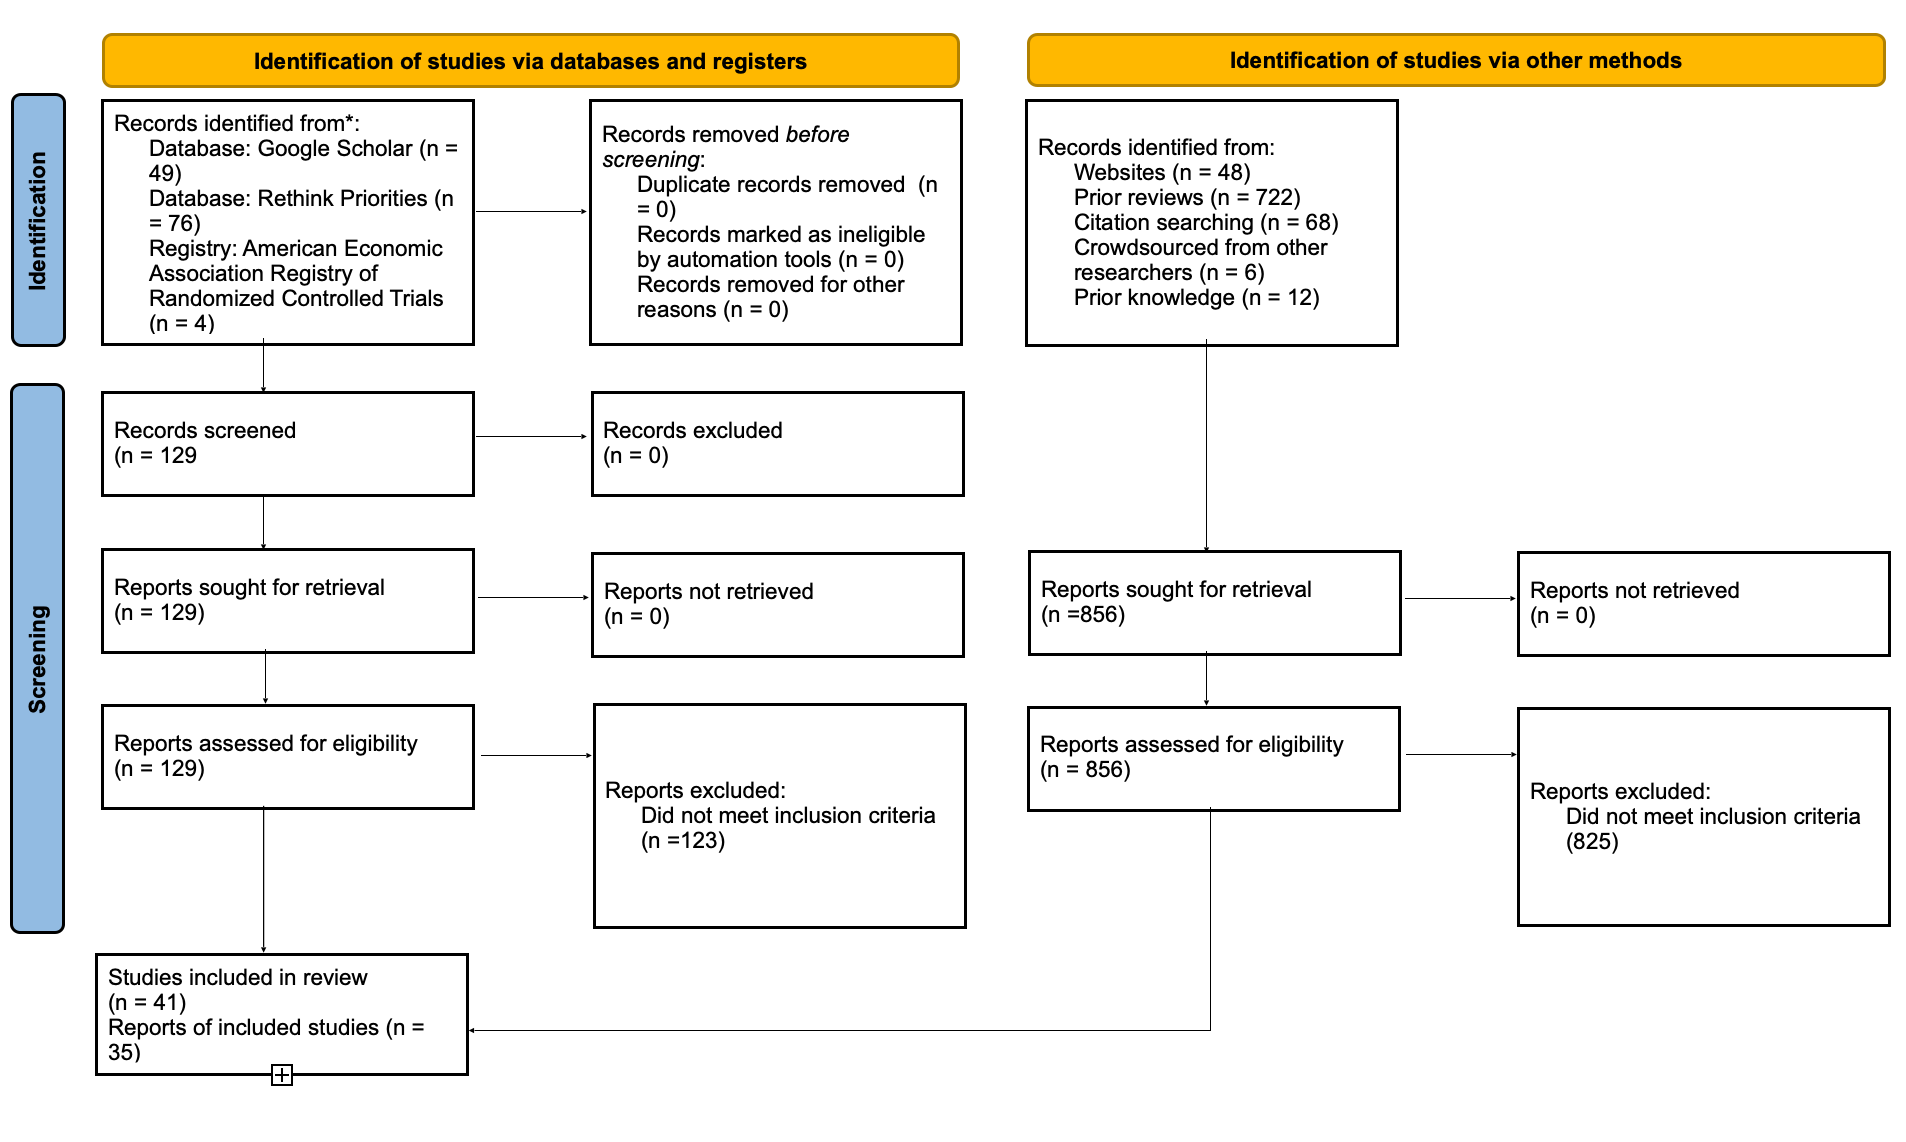
\includegraphics[width=1.2\linewidth,]{./figures/prisma-diagram} \end{center}

\subsection{Data extraction}\label{sec3.3}

The first author extracted all data. We extracted an effect size for one
outcome per intervention: the measure of net MAP or RPM consumption that
had the longest follow-up time after the intervention Additional
variables coded included information about publication, details of the
interventions, length of follow-ups, intervention theories, and
additional details about interventions' methods, contexts, and open
science practices (see accompanying code and data repository for full
documentation: ). When in doubt about calculating effect sizes, we
consulted publicly available datasets and/or contacted authors. To
assess risk of bias, we collected data on whether outcomes were
self-reported or objectively measured, publication status, and presence
of a pre-analysis plan and/or open data (table 3).

All effect size conversions were conducted by the first author using
methods and R code initially developed for previous papers
\citep{paluck2019, paluck2021, porat2024} using standard techniques
\citep{cooper2019}, with the exception of a difference in proportion
estimator that treats discrete events as draws from a Bernoulli
distribution (see appendix to \citep{paluck2021} for details). As our
measure of standardized mean difference, we used Glass's \(\Delta\)
whenever possible, defined as
\(\Delta = \frac{\mu_T - \mu_C}{\sigma_C}\), where \(\mu_T\) and
\(\mu_C\) respectively denote the treatment and control group means and
\(\sigma_C\) denotes the pre-treatment control group standard deviation.
We standardized on the SD of the control group at pre-treatment. If the
control group SD was not available, we standardized on the pooled SD.
When means and SDs were not available, we converted effect sizes
from:When means and SDs were not available, we converted effect sizes
from: regression coefficients, eta squared, or z-scores. When there was
insufficient information to calculate a specific SMD, but the text
reports the result as a null, we recorded the outcome as an
``unspecified null'' and set it to 0.01.

\subsection{Statistical analysis methods}\label{sec3.4}

Results were synthesized using robust variance estimation (RVE) methods
\citep{hedges2010} as implemented by the \texttt{robumeta} package
\citep{fisher2015} in \texttt{R} \citep{Rlang}. Many studies in our
sample featured multiple treatment groups compared to a single control
group. Therefore, we used the RVE method to allow for the resulting
dependence between observations, as well as a standard small-sample
correction.

Data analyses were largely conducted with custom functions building on
\texttt{tidyverse} \citep{wickham2019} We assessed publication bias
using selection model methods \citep{hedges1992, vevea1995}, sensitivity
analysis methods \citep{mathur2024}, and the significance funnel plot
\citep{mathur2020}. These methods assume that the publication process
favors ``statistically significant'' (i.e., p \textless{} 0.05) and
positive results over ``nonsignificant'' or negative results. Our
sensitivity check meta-analyzes only non-affirmative results, which
creates an estimate under a hypothetical ``worst-case'' publication bias
scenario where affirmative studies are almost infinitely more likely to
be published than non-affirmative studies. We conducted these analyses
using functions in \texttt{metafor} \citep{viechtbauer2010} and
\texttt{PublicationBias} \citep{mathur2020, mathur2024}.

We used \texttt{Rmarkdown} \citep{xie2018} and a containerized online
platform \citep{moreau2023, clyburne2019} to ensure computational
reproducibility \citep{polanin2020}.

\section{Discussion}\label{discussion}

Our overall effect of SMD = 0.07, as well as our upper confidence bound
of SMD = 0.12, lead us to conclude that reducing MAP consumption is an
unsolved problem. Effects were also consistently small across an array
of locations, study designs, and intervention categories. Some
individual studies found comparatively larger effects (SMD
\textgreater{} 0.5:
\citep{carfora2023, merrill2009, kanchanachitra2020, bianchi2022, piester2020}).
However, each builds on a fairly unique theory of change and employs
idiosyncratic methods. We view these these interventions as intriguing
candidates for subsequent research and replication, and conclude that no
theoretical approach, delivery mechanism, or intended persuasive message
should be considered a well-validated method of reducing MAP
consumption.

Though this may surprise readers of previous reviews
\citep{mathur2021meta, meier2022, mertens2022}, our divergent results
likely reflect our stricter methodological inclusion criteria. For
instance, of the ten largest effect sizes recorded in
\citep{mathur2021effectiveness}, nine measured attitudes and/or
intentions, and the tenth came from a non-randomized design. Prior
research has found that intentions often do not predict behavior
\citep{mathur2021effectiveness}, and reviews in other fields have found
systematic differences in impacts between randomized and non-randomized
evaluations \citep{porat2024, stevenson2023}. Our results raise the
possibility that previous reviews' positive findings might be largely
attributable to bias, though this will require further empirical
evaluation.

Another potentially surprising result is that very few (two) choice
architecture papers met our methodological inclusion criteria. Most
potentially eligible papers either measured hypothetical outcomes or
measured outcomes immediately after the intervention. Moreover, prior
reviews that found choice architecture approaches to be consistently
effective at modifying diet typically focused on foods that may have
weaker cultural and social attachments than MAP, such as sugary drinks
and snacks \citep{venema2020, adriaanse2009}. We speculate that people
are more likely to notice, and care, when the burger is missing from the
menu than when their soft drink is smaller.

Likewise, as our analyses show, studies aimed at reducing RPM
consumption are associated with a much larger effect size (SMD = 0.25)
than those aimed at reducing all MAP consumption. Sharply curtailing RPM
consumption is a core component of current leading dietary guidelines,
such as the heart-healthy diet \citep{diab2023}, but many of these same
guidelines encourage moderate intake of poultry and fish. Further,
reducing RPM consumption is frequently mentioned as something consumers
can and should do to personally fight climate change
\citep{auclair2024}. By contrast, vegetarianism is still a minority diet
worldwide \citep{tilman2014} that consumers consider to be difficult,
unsatisfying, and expensive \citep{bryant2019}. We speculate that
cutting back on RPM is perceived as easier and more likely to be
socially rewarded than is cutting back on MAP generally, and that this
explains the observed difference in effect sizes.

We caution that our analyses are limited by our small sample size. Our
moderation analysis, for instance, tests differences between studies
that are highly confounded, limiting our ability to detect the
independent association of a given variable with effect size. Further,
our meta-analytic database is a non-random sample of the literature writ
large, and our estimates of publication bias should not be taken as
estimates for the entire literature.

Most importantly, our results are highly sensitive to inclusion choices
about dependent variables, which arguably means they lack robustness.
However, this critique is a double-edged sword. Our paper suggests that
prior reviews' findings are also more sensitive to inclusion rules than
was previously known.

Overall, we are encouraged by positive trends in the literature. First,
as noted, a majority of studies in our meta-analysis have been published
since 2020, indicating the field's growing dedication to questions of
credible design and measurement. Second, we observe many fruitful
collaborations between researchers and advocacy organizations, as shown
by the plethora of nonprofit white papers in our sample. Third, many
promising designs and interventions yet await rigorous evaluation. For
instance, no study that met our criteria evaluated extended contact with
farm animals \citep{cerrato2022}, manipulations to the price of meat
\citep{wilde2016}, activating moral and/or physical disgust
\citep{palomo2018}, watching popular media such as the \emph{Simpsons}
episode ``Lisa the Vegetarian'' \citep{byrd2010} or the movie
\emph{Babe} \citep{novatna2019}, and many categories of choice
architecture intervention \citep{olafsson2024}. Moreover, we are
encouraged by contemporary research designs that offer creative
solutions to longstanding measurement challenges, for example by
implementing a default intervention at lunch and then measuring outcomes
at dinner as well to assess potential compensatory effects
\citep{vocski2024}.

In sum, though we view meaningfully reducing MAP consumption as an
unsolved problem, we see no reason to think it is unsolvable.

\bmhead{Acknowledgments}

\emph{Thanks to Alex Berke, Alix Winter, Anson Berns, Dan Waldinger,
Hari Dandapani, Adin Richards, Martin Gould, and Matt Lerner for
comments on an early draft. Thanks to Jacob Peacock, Andrew Jalil, Gregg
Sparkman, Joshua Tasoff, Lucius Caviola, Natalia Lawrence, and Emma
Garnett for help with assembling the database and providing guidance on
their studies. Thanks to Sofia Vera Verduzco for research assistance. We
gratefully acknowledge funding from the NIH (grant R01LM013866), Open
Philanthropy, and the Food Systems Research Fund (Grant FSR
2023-11-07).}

\section*{Declarations}\label{declarations}
\addcontentsline{toc}{section}{Declarations}

\section{Supplement}\label{Sec5}

\subsection{Description of code and data
repository}\label{description-of-code-and-data-repository}

Our code and data are shared on the Open Science Framework {[}LINK{]},
GitHub {[}LINK, and Code Ocean {[}LINK{]}. Our main document,
\texttt{MAP-reduction-meta.Rmd}, reproduces this paper, with every
quantitative claim (as well as the first two figures) reproduced each
time the document is knit.

Our included datasets are

\begin{itemize}
\item
  \texttt{vegan-meta.csv}, our primary meta-analytic dataset;
\item
  \texttt{rpmc-data.csv}, our secondary dataset of studies aimed at
  reducing consumption of RPM;
\item
  \texttt{robustness-data.csv}, another secondary dataset borderline
  studies for a robustness check (see section below);
\item
  \texttt{review-of-reviews.csv}, which details the the 157 reviews we
  consulted;
\item
  \texttt{excluded-studies.csv}, which details the papers we screened
  but did not include, along with their reasons for exclusion and where
  we found them (the studies in \texttt{robustness-data.csv} are
  included in this dataset as well).
\end{itemize}

The repositories have more details about the included scripts and
supplementary materials (e.g.~licenses).

\subsection{Robustness to less stringent inclusion
criteria}\label{Sec5.1.1}

We coded and meta-analyzed a supplementary dataset of 22 studies,
comprising 35 point estimates, that feature many strong design features
but that were excluded for one of five reasons: 1) issues with random
assignment or the control group (for instance, where the control group
receives some aspect of treatment \citep{piazza2022}, or where treatment
was alternated weekly but not randomly \citep{garnett2020}); 2)
underpowered (too few clusters \citep{reinders2017} or subjects
\citep{lentz2019}); 3) immediate outcome measurement
\citep{dannenberg2023, sparkman2017, griesoph2021, hansen2021}; 4)
actively encouraging substitution within categories of MAP, e.g.~from
red meat to fish \citep{celis2017, johansen2009}; or 5) uncertainty in
calculating an effect size arising from missing information about the
behavior of diners who opt out of treatment to avoid a vegetarian meal
\citep{betterfoodfoundation2023}.

Taken together, our integrated dataset including both our main sample
and this supplementary one yields a pooled effect of SMD = 0.2 (95\% CI:
{[}0.09, 0.31{]}), p = 0. Particularly large results were found in
studies that measured outcomes immediately \citep{hansen2021} or that
had smaller samples \citep{lentz2020}.

\subsection{Robustness to an alternative estimation
method}\label{Sec5.1.2}

Our pre-analysis plan (\url{https://osf.io/3sth2}) used a model from
\texttt{metafor} to analyze a synthetic dataset. However, as we
assembled the actual dataset, we noticed that many papers had, across
interventions, non-independent observations, typically in the form of
multiple treatments compared to a single control group. Upon discussion,
the team's statistician (MBM) suggested that the \texttt{CORR} model
from the \texttt{robumeta} package, a robust variance estimation (RVE)
method, would be a better fit.

Using our original estimation strategy from \texttt{metafor}, we detect
a pooled effect size of 0.04 (95\% CI: {[}-0.02, 0.1{]}), p = 0.1600299.
(Although \texttt{metafor} also provides an RVE estimator, it applies
the correction to the standard errors and not to the overall estimate,
and we preferred a model that incorporates clustering information at the
level of effect estimation.)

\subsection{Robustness to a stricter definition of
delay}\label{Sec5.1.3}

\begin{Shaded}
\begin{Highlighting}[]
\NormalTok{strict\_delay\_model }\OtherTok{\textless{}{-}}\NormalTok{ dat }\SpecialCharTok{|\textgreater{}} \FunctionTok{filter}\NormalTok{(delay\_post\_endline }\SpecialCharTok{\textgreater{}} \DecValTok{0}\NormalTok{) }\SpecialCharTok{|\textgreater{}} \FunctionTok{extract\_model\_results}\NormalTok{()}
\end{Highlighting}
\end{Shaded}

Our delay-related inclusion criterion aimed to limit our analysis to
enduring effects. We were concerned that subjects who are encouraged to
have a single vegetarian meal might later compensate by consuming more
MAP at the next one, which would make an immediate outcome measurement
an upwardly biased estimate of overall effects.

Upon reviewing studies, however, we found that numerous high-quality
studies modified eating environments over multiple days and did not
incorporate a delayed measure following the \emph{final} day of
treatment. For example, \citep{andersson2021} included 50 combined days
of treatment and control, but the interval between treatment and any
individual outcome measurement was zero days. By one light, such studies
lack delayed outcome measures. In another, the multi-day setup in a
single environment allows for theoretical delay so long as participants
can return to the site of treatment and have their meal choices
evaluated multiple times.

We decided to include multi-day studies where delayed outcomes were at
least possible through repeat visits by subjects to the intervention
site. Our delay variable therefore reflects the days elapsed from the
beginning of treatment, rather than its conclusion, to measurement.

We also coded a secondary delay variable that corresponds to time
elapsed between treatment \emph{conclusion} to measurement. Restricting
our analysis to the 31 studies and 96 point estimates where this
secondary delay exceeds zero, we observe an effect of SMD = 0.07 (95\%
CI: {[}0.01, 0.12{]}), p = .028.

\subsection{Notes on search strategy}\label{Sec5.2}

\begin{comment} we could take the next few paragraphs out and start with the sentence "we employed what could be called a "prior-reviews-first" search strategy."
\end{comment}

Our search process was shaped by three unusual features of our research
project. First, our surveyed literature was highly interdisciplinary,
with few shared terms to describe itself. For instance, the term `MAP'
is not universally agreed upon; other papers use animal-based protein,
edible animal products, or just meat, while others focus on a
particular, sometimes unusual category of MAP, such as fish sauce
\citep{kanchanachitra2020}, or discussed their agenda mainly in terms of
increasing plant-based alternatives. Coming up with an exhaustive list
of terms to search for from first principles would have been, in our
opinion, virtually impossible.

Second, our methods-based inclusion criteria complicated screening on
titles and abstracts. While it was sometimes possible to use solely that
information to eliminate studies with no interventions
(e.g.~survey-based research), determining whether an intervention
qualified almost always required some amount of full text screening. We
also discovered that terms like ``field experiment'' have varying
meanings across papers, and identifying whether a measured food choice
was hypothetical or not often required a close reading. For these
reasons, screening thousands or tens of thousands of papers struck us as
prohibitively time-consuming.

Third, we found an extraordinary number of prior reviews, typically
aimed at one disciplinary strand or conceptual approach, touching on our
research question. Reviewing tables and bibliographies of those papers
proved enormously fruitful for both assembling our dataset and getting a
sense of the broader literature.

For these reasons, we employed what could be called a
``prior-reviews-first'' search strategy. Of the 985 papers we reviewed,
a full 73 \% of all manuscripts we screened came from prior reviews, and
43 \% of papers in our main dataset. (See the next section of the
supplement for notes on reviews that were especially informative.) Then,
as detailed in the main text, we employed a multitude of other search
strategies to fill in our dataset, one of which was systematic search.
In particular, we searched Google Scholar for the following list of
terms, and checked ten pages of results for each:

\begin{itemize}
\tightlist
\item
  ``dynamic'' ``norms'' ``meat''
\item
  ``dynamic'' ``norms'' ``meat'' ``consumption''
\item
  ``field'' ``experiment'' ``plant-based''
\item
  ``meat'' ``alternatives'' ``default'' ``nudge''
\item
  ``meat'' ``consumption'' ``reducing'' ``random''
\item
  ``meat'' ``purchases'' ``information'' ``nudge''
\item
  ``meat'' ``reduction'' ``randomized''
\item
  ``meat'' ``sustainable'' ``random''
\item
  ``nudge'' ``meat'' ``default''
\item
  ``nudge'' ``reduce'' ``meat'' ``consumption''
\item
  ``nudge'' ``sustainable'' ``consumption'' ``meat''
\item
  ``nudge'' ``theory'' ``meat'' ``purchasing''
\item
  ``norms'' ``animal'' ``products''
\item
  ``nudges'' ``norms'' ``meat''
\item
  ``random'' ``nudge'' ``meat''
\item
  ``randomized controlled trial'' ``meat'' ``consumption'' ``reduce''
\item
  ``sustainable'' ``meat'' ``nudge''
\item
  ``sustainable'' ``meat'' ``nudge'' ``random''
\item
  ``university'' ``meat'' ``default'' ``reduction''
\end{itemize}

Additionally, we searched the American Economic Association's RCT
registry for the the terms ``meat'' and ``random'' and reviewed all
matching results in the relevant time frame.

Another unconventional part of our search strategy was our use of of an
AI-based search tool (\url{https://undermind.ai/}), to which we
described our research question and then reviewed 100 results that it
generated. This yielded one paper that met our inclusion criteria
\citep{mattson2020} that seems to have slipped past many other
systematic search processes.

Finally, we benefited from two in-progress literature reviews at Rethink
Priorities, ``a think-and-do tank'' that researches animal welfare as
one of its four main priorities. Both of these literature reviews are
aimed at assessing interventions that reduce MAP consumption, but have
broader inclusion criteria than our paper employed. For more details on
these two projects, see \url{<https://osf.io/74paj>} and
\url{<https://meat-lime.vercel.app>}.

\subsection{Discussion of prior
reviews}\label{discussion-of-prior-reviews}

We turn now to a selective overview of prior reviews that were highly
relevant to this one.

Among the reviews that found MAP reduction interventions to be
effective, several focused exclusively on choice architecture.
\citep{arno2016} found that nudges led to an average increase of healthy
dietary choices of 15.3\%, while \citep{byerly2018} found that
committing to reduce meat intake and making menus vegetarian by default
were more effective than educational interventions. However, the vast
majority of vegetarian-default studies we analyzed for this paper did
not qualify for our analysis because they lacked delayed outcomes. In a
similar vein, \citep{mertens2022} concludes that food choices are
``particularly responsive to choice architecture interventions'' (p.~1),
but featured no studies that met our inclusion criteria.

\citep{bianchi2018restructuring} found that reducing meat portions,
making alternatives available, moving meat products to be less
conspicuous, and changing meat's sensory properties can all reduce meat
demand. \citep{pandey2023} found that changing the presentation and
availability of sustainable products was effective in increasing demand
for them.

In a meta-review, \citep{grundy2022} found environmental education to be
especially promising, with substantial evidence also supporting health
information, emphasizing social norms, and decreasing meat portions.

Some reviews have focused on particular settings for MAP reduction
interventions. \citep{hartmannboyce2018} found that grocery store
interventions, such as price changes, suggested swaps, and changes to
item availability, were effective at changing purchasing choices.
However, that review covered a wide variety of health interventions,
such as reducing consumption of dietary fat and increasing fruit and
vegetable purchases. It is unclear how directly such findings translate
to MAP reduction efforts. Meanwhile, \citep{chang2023} focused on
university meat-reduction interventions and found more promising results
than did reviews that looked at the wider public. \citep{harguess2020}
reviewed 22 studies on meat consumption and found promising results for
educational interventions focused on the environment, health, and animal
welfare. That paper recommends using animal imagery to cause an
emotional response and utilizing choice architecture interventions. Our
review, by contrast, found no relationship between animal welfare
appeals and MAP consumption.

Taking a different angle, \citep{adleberg2018} reviewed the literature
on protests in a variety of movements and found mixed evidence of
efficacy. The authors recommend that animal advocacy protests have a
specific target (e.g.~a particular institution) and ``ask.''

Other reviews assesed which groups are most easily influenced by
interventions to reduce MAP consumption. For example,
\citep{blackford2021} found that nudges focused on ``system 1'' thinking
were more effective at encouraging sustainable choices than those
focused on ``system 2,'' and that interventions had greater effects on
females than males. Our review also featured studies showing differences
between men and women.

\citep{rosenfeld2018} reports that meat avoidance is associated with
liberal political views, feminine gender, and higher openness,
agreeableness and neuroticism. That review also identifies challenges
and barriers to vegetarianism, such as recidivism and hostility from
friends and family. Future research could tailor interventions to
address these barriers.

Several reviews have had mixed or inconclusive results. For instance,
\citep{bianchi2018conscious} found that health and environmental appeals
appear to change dietary intentions in virtual environments, but did not
find evidence of actual consumption changes. Likewise,
\citep{kwasny2022} notes that most existing research focuses on
attitudes and intentions and lacks measures of actual meat consumption
over an extended period of time. \citep{taufik2019} reviewed many
studies aimed at increasing fruit and vegetable intake, but found far
fewer that looked at reducing MAP consumption. \citep{benningstad2020}
found that dissociation of meat from its source plays a role in meat
consumption, but no extant research that included behavioral outcomes.

A few reviews have found evidence that seems to recommend against
particular interventions. \citep{greig2017} reviewed the literature on
leafleting for vegan/animal advocacy outreach, and observed biases that
may have led to overestimated impacts. That paper concluded that
leafleting does not seem cost-effective, though with significant
uncertainty. This accords with our findings on advocacy organization
materials' limited effects.

\citep{nisa2019} meta-analyzed interventions to improve household
sustainability, of which reducing MAP consumption was one of several.
Although they found small effect sizes for most interventions, they
concluded that nudges were comparatively effective, as did
\citep{ensaff2021}. Similarly, \citep{rau2022} reviewed the literature
on environmentally friendly behavior changes, including but not limited
to diet change, and found small or nonexistent effects in most cases.
Only fifteen interventions in that paper were described as ``very
successful,'' and none of these related to food.

Finally, we note a few papers that were helpful in filling out our
supplementary datasets. \citep{ronto2022} investigated interventions to
move consumer to protein sources with lower ecological footprints, and
was instrumental in filling out our RPM and robustness check datasets,
as were \citep{kwasny2022} and \citep{grummon2023}.

Our overall conclusion from these 150+ papers is that the marginal value
of a new rigorous evaluation is much higher than that of a new
systematic review. We also encourage researchers to be cautious in
extrapolating impacts across outcome categories. For instance, many
reviews concluded that choice architecture approaches are effective at
changing food choice, but these are typically aimed at foods with weak
social and cultural associations. Whether these interventions work for
something as fraught with meaning as meat remains to be seen.

\newpage

\renewcommand\refname{References}
\bibliography{./vegan-refs.bib}


\end{document}
